\documentclass[9pt]{article}
\usepackage{siunitx,gensymb} % gensym gives degree
\usepackage{amsmath}
\usepackage{newtxtext,newtxmath}
\usepackage[numbers]{natbib}
\usepackage{graphicx}
\usepackage{xcolor}
\usepackage[bookmarks=true,bookmarksnumbered=true,hidelinks]{hyperref}
\usepackage{cleveref}
\usepackage[margin=1in]{geometry}
\usepackage[compact]{titlesec}

% --- Math ---
\newcommand{\pp}[2]{\frac{\partial #1}{\partial #2}}
\newcommand{\ppt}[2]{\frac{\partial^2 #1}{\partial #2^2}}
\newcommand{\pptt}[2]{\frac{\partial^3 #1}{\partial #2^3}}
\newcommand{\ppttt}[2]{\frac{\partial^4 #1}{\partial #2^4}}
\newcommand{\DD}[2]{\frac{D #1}{D #2}}
\newcommand{\dd}[2]{\frac{d #1}{d #2}}
\newcommand{\ddt}[2]{\frac{d^2 #1}{d #2^2}}
\newcommand{\ddtt}[2]{\frac{d^3 #1}{d #2^3}}
\newcommand{\ddttt}[2]{\frac{d^4 #1}{d #2^4}}
\newcommand{\mbb}[1]{\mathbb{#1}}    % math blackboard
\newcommand{\mbf}[1]{\mathbf{#1}}
\newcommand{\mrm}[1]{\mathrm{#1}}
\newcommand{\mcal}[1]{\mathcal{#1}}  % math calligraphy
\newcommand{\mbfh}[1]{\widehat{\mathbf{#1}}}
\newcommand{\mbfv}[1]{\vec{\mathbf{#1}}}
\newcommand{\half}{\frac{1}{2}}
\newcommand{\third}{\frac{1}{3}}
% --- Equations ---
\newcommand{\be}{\begin{eqnarray}}
\newcommand{\ee}{\end{eqnarray}}
\newcommand{\ben}{\begin{eqnarray*}}
\newcommand{\een}{\end{eqnarray*}}
% --- Numerical methods ---
\newcommand{\dx}{d\mbf{x}}
\newcommand{\Dt}{\Delta t}
\newcommand{\ih}{\hat{i}}
\newcommand{\jh}{\hat{j}}
\newcommand{\kh}{\hat{k}}
\newcommand{\nh}{\hat{n}}
\newcommand{\xh}{\hat{x}}
\newcommand{\yh}{\hat{y}}
\newcommand{\zh}{\hat{z}}
\newcommand{\uj}[1]{u_{j  #1 }}
\newcommand{\ujn}[2]{u_{j  #1 }^{n  #2}}
\newcommand{\BigO}{\mathcal{O}}
\newcommand{\CFL}{{\mbox{CFL}}}
\newcommand{\opt}[1]{#1 (x^{\star})}
% --- Flow ---
\newcommand{\Uinf}{U_{\infty}}
\newcommand{\Vinf}{V_{\infty}}
\newcommand{\Minf}{M_{\infty}}
\newcommand{\bVinf}{\mbf{V}_{\infty}}
\newcommand{\pinf}{p_{\infty}}
\newcommand{\cpmin}{C_{p_{\tn{min}}}}
% --- Other Shorthands ---
\newcommand{\tn}[1]{\textnormal{#1}}
\newcommand{\fw} {forward swept\:}
\newcommand{\un} {unswept\:}
\newcommand{\bw} {backward swept\:}
\newcommand{\scriptth}{\scriptsize \textnormal{th}}
\newcommand{\cfrp}[1] {CFRP #1$^\circ$\:}
\newcommand{\tss}[1]{\textsuperscript{#1}}
\newcommand{\wrt} {with respect to\:}

% --- Spacings ---
\setlength{\headsep}{0.0in}
\setlength{\topmargin}{0.0in}
\setlength{\textheight}{8.8in}
\setlength{\textwidth}{6.8in}
\setlength{\oddsidemargin}{-.15in}
\setlength{\evensidemargin}{-.15in}
\setlength{\unitlength}{1in}

\bibliographystyle{unsrtnat}


\begin{document}

\title{\vspace{-1.5cm} DCFoil Documentation}
\author{Galen W.~Ng}
\maketitle
% ==============================================================================
%                         BEGIN
% ==============================================================================
\section*{Summary}
% 
DCFoil is a program for the dynamic analysis and design optimization of composite hydrofoils.
\begin{figure}[htbp!]
    \centering
    % reference: trim={<left> <lower> <right> <upper>}
    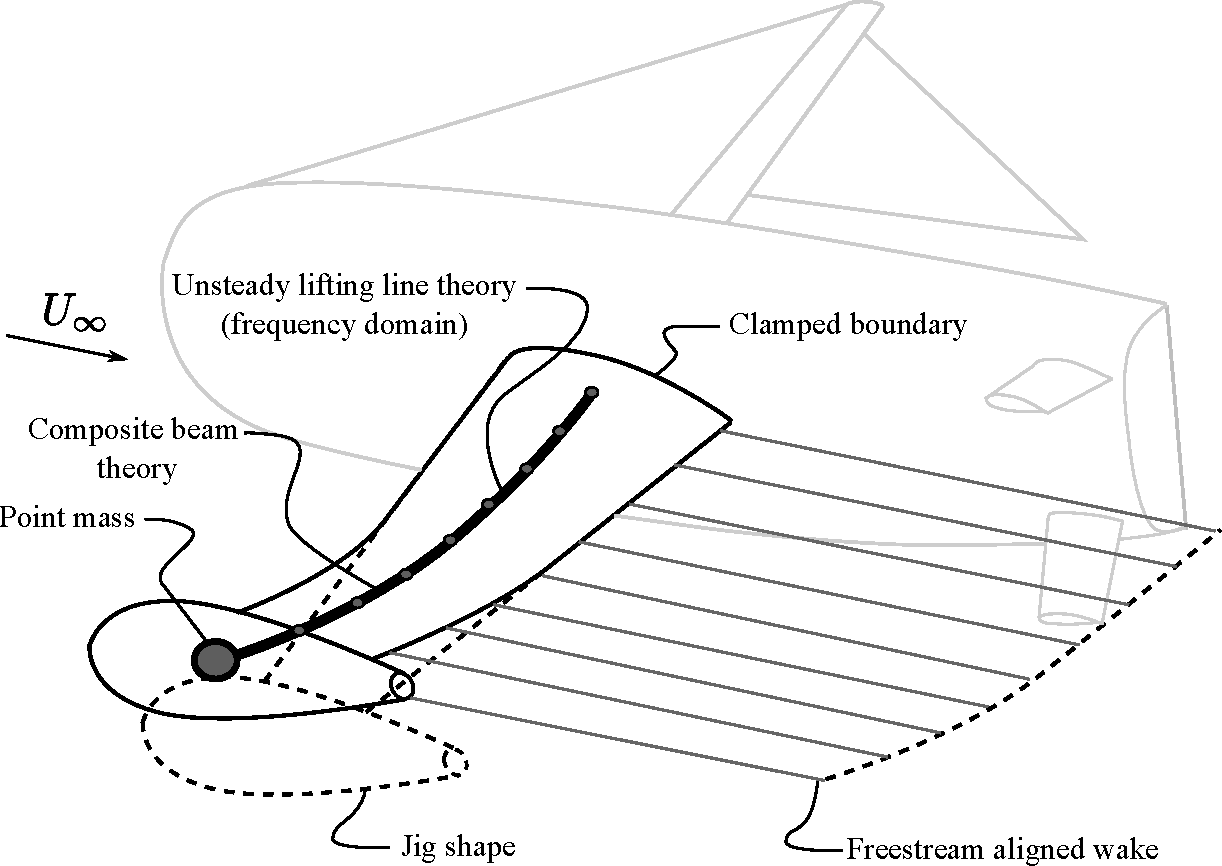
\includegraphics[width=0.7\linewidth,clip,trim={0cm 0cm 0cm 0cm}]{keel-dcfoil.pdf}
    \caption{\label{fig:keel-dcfoil}
        DCFoil modeling approach
    }
\end{figure}

\clearpage
\tableofcontents
\clearpage
%------------------------------------------------------------------------------
\section{Coordinate system}
% 
Flow is in the $x$-direction, span is in the $y$-direction, and the vertical direction is $z$.
%------------------------------------------------------------------------------
\section{Discretization}
\subsection{Structural model}
% 
The local beam model uses the spanwise direction as $x$ (subscript 1), the chordwise direction as $y$ (subscript 2), and the vertical direction as $z$ (subscript 3).
It is transformed to the global coordinate system by the rotation matrices.
\subsubsection{Beam finite element}
% 
The composite beam model uses the well-known slender beam parameters $EI_s$, $GJ_s$, $EA_s$, and additionally $S_s$ and $K_s$ to account for structural warping of non-circular cross sections and material bend-twist coupling, respectively.
% 
\subsubsection{Constitutive relations for composite beams}
% 
The beam parameters are computed from classical lamination theory (CLT) for composite plates using the high aspect ratio plate model from \citet{Weisshaar1985}.
\be
EI = c\left( D_{11} - \frac{D_{12}^2}{D_{22}}\right)      , \quad
GJ = 4c \left(D_{66} - \frac{D_{26}^2}{D_{22}}\right)     , \quad
K  = 2c \left(D_{16} - \frac{D_{26}D_{12}}{D_{22}}\right)
\ee
These relations do not restrict chordwise rigidity (camber), but they do assume zero chordwise moment.
\citet{LOTTATI1985} used the chordwise rigid relations, which simplifies the algebra.

The flexural stiffnesses $D_{ij}$ come CLT via
\begin{align}
    D_{11} & = Q_{11}\cos^4(\theta_f)+2\left( Q_{12}+2Q_{66}\right)\sin^2(\theta_f)\cos^2(\theta_f)+Q_{22}\sin^4(\theta_f)                             \\
    D_{22} & = Q_{11}\sin^4(\theta_f)+2\left( Q_{12}+2Q_{66}\right)\sin^2(\theta_f)\cos^2(\theta_f)+Q_{22}\cos^4(\theta_f)                             \\
    D_{66} & = \left(Q_{11} +Q_{22} - 2Q_{12}-2Q_{66}\right)\sin^2(\theta_f)\cos^2(\theta_f)+Q_{66}\left( \sin^4(\theta_f)+\cos^4(\theta_f) \right)    \\
    D_{12} & = \left(Q_{11} +Q_{22} - 4Q_{66}\right)\sin^2(\theta_f)\cos^2(\theta_f) + Q_{12}\left( \sin^4(\theta_f)+\cos^4(\theta_f) \right)          \\
    D_{16} & = \left(Q_{11} +Q_{22} - 2Q_{66}\right)\sin(\theta_f)\cos^3(\theta_f) + \left(Q_{12}-Q_{22}+2Q_{66}\right) \sin^3(\theta_f)\cos(\theta_f) \\
    D_{26} & = \left(Q_{11} +Q_{22} - 2Q_{66}\right)\sin^3(\theta_f)\cos(\theta_f) + \left(Q_{12}-Q_{22}+2Q_{66}\right) \sin(\theta_f)\cos^3(\theta_f) 
\end{align}
%
The reduced in-plane stiffness coefficients $Q_{ij}$ for the individual plies are
%
\be
Q_{11} = \frac{E_1}{1-\nu_{12}\nu_{21}}, \quad
Q_{12} = \frac{\nu_{12} E_2}{1-\nu_{12}\nu_{21}}, \quad
Q_{22} = \frac{E_2}{1-\nu_{12}\nu_{21}}, \quad
Q_{66} = G_{12}
\ee

\subsection{Hydrodynamic loads}
% 
\subsubsection{Steady lifting line}
% 
The lifting line model derives from~\citet[Ch. XI]{Glauert1983a} and works for arbitrary chord.
Specifically, we are after sectional lift slopes ($\textstyle c_{\ell_\alpha} = dc_\ell/d\alpha = a_0$).
We assume
\begin{itemize}
    \item the chord is small compared to the span,
    \item the wing is symmetric about the centerline,
    \item span is straight and orthogonal to the freestream
    \item trailing vortices are shed from the trailing edge and align with the freestream (no sweep or dihedral)
\end{itemize}

The wing is represented by superimposing ``horseshoe'' systems of vortex lines (analagous to a wire with electrical current).
This is because the circulation across a wing is not constant.
The free vortex system is a sheet of trailing vortices springing from the trailing edge.
The induced velocity of an element of the line ($ds$) at point $P$ from one vortex line of constant strength $\Gamma$ is
\be
dq = \frac{\Gamma}{4 \pi r^2} \sin(\theta) ds
\ee
but in practice, one would solve this is an integral over the entire vortex line, so we will build up to the full wing.

% We know the forces to be
% \begin{align}
%      & L = \int_{-s/2}^{s/2} \rho \Uinf \Gamma(y) dy          \\
%      & D_i = \int_{-s/2}^{s/2} \rho \Uinf w(y)  \Gamma(y) dy
% \end{align}
% where $s$ is total span.
To begin solution, we first assume the circulation is the Fourier series\footnote{\citet{Kerwin2010} use $\tilde{y}$ as $\theta$}
\be
\Gamma(y) = 2 \Uinf s \sum_{n=1}^{\infty} a_n \sin \left( n \theta \right)
\quad \tn{where }
y = -\frac{s}{2}\cos(\theta)
\quad \tn{and }
\theta \in \left[-\frac{\pi}{2},\frac{\pi}{2}\right]
.
\ee
The difficulty is now determining the Fourier coefficients $a_n$ so we need some relations for $\Gamma(y)$ to solve it.

One relation is the equation for the normal induced velocity (downwash velocity) at a point along the span
\be
\label{eq:downwash}
w(y) = \frac{1}{4\pi}
\int_{-s/2}^{s/2} \frac{\dd{\Gamma}{\eta} }{y - \eta} d\eta
=
\boxed{
    -\Uinf \sum_{n=1}^{\infty} \frac{n a_n \sin \left( n \theta \right)}{\sin(\theta)}
}
\ee
where $\eta$ is the spanwise coordinate and $s$ is total span.
We skipped a few steps in the derivation~\cite[Sec.~3.7]{Kerwin2010}.

The second relation is from sectional lift as a function of circulation.
Recall that the circulation at a section (derived from Kutta-Joukowski lift theorem) is
\be
\label{eq:circulation}
\Gamma(y) = \half c_\ell c \Uinf
=\half a_0 c \left(\Uinf \alpha - w(y)\right)
\ee
where we made use of $c_\ell = a_0 \alpha_{\tn{eff}} = a_0 \left(\alpha - w/\Uinf\right)$.
After substitution of the Fourier series form and combining Equations~\eqref{eq:downwash} and~\eqref{eq:circulation}, we end up with
\be
\label{eq:circulation2}
\sum_{n=1}^{\infty} a_n \sin(n\theta) \left(n\mu + \sin(\theta)\right)
=
\mu \alpha \sin(\theta)
\quad \tn{where }\mu(\theta) = \frac{a_0 c(\theta)}{ 4 s}
\ee

Here's the digestion of the Julia code which does the numerical solution of Equation~\eqref{eq:circulation2} but symmetrically about the centerline.
\begin{align*}
     & \tilde{y} = \left[
        0,\frac{\pi}{2}
        \right] \quad \tn{of size nNodes}
    \\
     & \mbf{n} = \left[1:2:2\times\tn{nNodes}\right]
    \\
     & \mbf{c} = c  \sin(\tilde{y}) \quad \tn{(parametrized vector leading to elliptical planform)}
    \\
     & \mbf{b} = \frac{\pi}{4} \frac{\mbf{c}}{s/2} \alpha \sin(\tilde{y}) \quad \tn{(RHS of Equation~\eqref{eq:circulation2} in vector form)}
    \\
     & \tilde{y}n = \tilde{y} \otimes \mbf{n} \quad \tn{(outer product)}
    \\
     & \mbf{A_0} = \begin{bmatrix}
                       |               & |                        \\
                       \sin(\tilde{y}) & \sin(\tilde{y}) & \cdots \\
                       |               & |
                   \end{bmatrix} \quad \tn{(square matrix of $\sin(\tilde{y})$)}
    \\
     & \mbf{A_1} = \frac{\pi}{4} \frac{\mbf{c}}{s/2} \otimes \mbf{n} \quad \tn{(outer product representing $n\mu$ on LHS)}
    \\
     & \mbf{A} = \sin(\tilde{y} n ) \odot \left( \mbf{A_0}+\mbf{A_1} \right)                                                                  \\
     & \mbf{A}\mbf{x} = \mbf{b} \quad \tn{(solve linear system for $\mbf{x} = a_n$)}                                                          \\
     & \Gamma(y) = 4 \Uinf s/2 \left(\underbrace{\sin(\tilde{y}n)\mbf{x} }_{\tn{mat-vec product}} \right)                                     \\
     & c_\ell = \frac{2\Gamma(y)}{\Uinf {c}}                                                                                                  \\
     & c_{\ell_{\alpha}} = \frac{c_\ell}{\alpha}
\end{align*}

\subsubsection{Extension to unsteady frequency domain}
% 
We are interested in the sectional lift and moments for a harmonically oscillating body.
\citet{Theodorsen:1934} came up with the Theodorsen function $C(k)$ to account for the lag and deficit in forces.
It is applied as a transfer function to the static hydrodynamics.
\begin{eqnarray}
    \label{eqn:GenFluidTheod}
    \left\{\begin{matrix}
        F_z \\
        M_y
    \end{matrix}\right\}_i =
    -
    \left(
    \left[
        \mbf{m_f}
        \left\{
        \begin{matrix}
            \ddot{w} \\
            \ddot{\psi}
        \end{matrix}
        \right\}
        \right]_i
    +
    \left[
        \mbf{c_f}
        \left\{\begin{matrix}\dot{w} \\ \dot{\psi} \end{matrix}\right\}
        \right]_i
    +
    \left[
        \mbf{k_f}
        \left\{\begin{matrix}w \\ \psi + \alpha_0 \end{matrix}\right\}
        \right]_i
    +
    \left[
        \mbf{\hat{c}_f}
        \left\{\begin{matrix}\dot{w}' \\ \dot{\psi}' \end{matrix}\right\}
        \right]_i
    +
    \left[
        \mbf{\hat{k}_f}
        \left\{\begin{matrix}w' \\ \psi' \end{matrix}\right\}
        \right]_i
    \right)
    \Delta y_i
\end{eqnarray}
where $\Delta y_i$ is the strip width at node $i$, which we assume to be equal to element length.
% 
\begin{equation}
    \label{eqn:FluidMass}
    \mbf{m_f} = \pi \rho_f b^2 \begin{bmatrix}
        1  & ab                                \\
        ab & b^2\left(\frac{1}{8} + a^2\right)
    \end{bmatrix}
\end{equation}
%
\begin{equation}
    \label{eqn:FluidDamp}
    \mbf{c_f}(k) =
    \frac{1}{2}\rho_f b U_0
    \left(
    \begin{aligned}
            \cos(\Lambda)
            \begin{bmatrix}
                \vspace{3mm}c_{\ell_{\alpha}} 2 C(k) & -b \left[2 \pi + c_{\ell_{\alpha}} (1-2a) C (k)\right]     \\
                c_{\ell_{\alpha}} eb 2C(k)           & \frac{b}{2} (1-2a)(2 \pi b - c_{\ell_{\alpha}} 2 eb C (k))
            \end{bmatrix}
            % + \\
            % \sin(\Lambda)\frac{\partial}{\partial y}
            % \begin{bmatrix}
            %     \vspace{3mm}2 \pi b & 2 \pi ab^2                           \\
            %     2\pi ab^2           & 2\pi b^3\left(\frac{1}{8}+a^2\right)
            % \end{bmatrix} % NOTE: this is a repeat of what is in c_f
        \end{aligned}
    \right)
\end{equation}
%
\begin{equation}
    \label{eqn:FluidStiff}
    \mbf{k_f}(k) = \frac{1}{2}\rho_f U_0^2 \cos(\Lambda)
    \left(
    \begin{aligned}
            \cos(\Lambda)
            \begin{bmatrix}
                0 & -C(k)2b c_{\ell_{\alpha}}     \\
                0 & -2eb^2 c_{\ell_{\alpha}} C(k)
            \end{bmatrix}
        \end{aligned}
    \right)
\end{equation}
%
\be
\label{eqn:FluidSweep}
\mbf{\hat{c}_f}(k) =
\frac{1}{2}\rho_f b U_0
\sin(\Lambda)
\left(
\begin{aligned}
        \begin{bmatrix}
            \vspace{3mm}2 \pi b & 2 \pi ab^2                           \\
            2\pi ab^2           & 2\pi b^3\left(\frac{1}{8}+a^2\right)
        \end{bmatrix}
    \end{aligned}
\right)
\ee
%
\begin{eqnarray}
    \mbf{\hat{k}_f}(k) =
    \frac{1}{2}\rho_f b U_0
    \sin(\Lambda)
    \left(
    \begin{aligned}
            U_0 \cos(\Lambda)
            \begin{bmatrix}
                \vspace{3mm} c_{\ell_{\alpha}}2 C (k) & - c_{\ell_{\alpha}} b (1-2a)C(k)          \\
                2ebc_{\ell_{\alpha}} C (k)            & \pi b^2  -c_{\ell_{\alpha}}eb^2(1-2a)C(k)
            \end{bmatrix}
        \end{aligned}
    \right)
\end{eqnarray}
% 
The extra $\hat{\square}$ matrices account for sweep effects on the quasi-steady (damping and stiffness) aerodynamics and are lumped into their respective global matrices if they are in phase with velocity or displacements.
%------------------------------------------------------------------------------
\section{Static solution}

%------------------------------------------------------------------------------
\section{Forced vibration solution}

%------------------------------------------------------------------------------
\section{Flutter solution}
\subsubsection{Mode space reduction}
%
To reduce the problem size, we use mode space reduction to a reduced set of $N_r$ generalized coordinates.
The displacement field is approximated by
%
\be
\mbf{u} \approx \mbf{Q}_r(y) \mbf{q}(t)
\ee
%
where $\mbf{q} \in \mathbb{R}^{N_r}$ is a vector of retained generalized coordinates and $\mbf{Q}_r \in \mathbb{R}^{N_s \times N_r}$ is a matrix with columns corresponding to eigenvectors.
This is typically called the normal mode method.
One then solves the eigenvalue problem
%
\be
\left( \mbf{K_s} - \omega_i^2 \mbf{M_s}
\right)
\widebar{  \mbf{u} }_i = 0
\ee
%
where $\omega_i$ is the natural frequency.
We compute $\widebar{  \mbf{u} }_i$ and collect them in the matrix
%
\be
\mathbf{Q}_r=\left[\begin{array}{cccc}
        \mid                    & \mid                    &        & \mid                        \\
        \overline{\mathbf{u}}_1 & \overline{\mathbf{u}}_2 & \cdots & \overline{\mathbf{u}}_{N_r} \\
        \mid                    & \mid                    &        & \mid
    \end{array}\right]
.
\ee
%
Now the reduced stiffness and mass matrices are
%
\be
\mbf{M_s}_r = \mbf{Q}_r^T \mbf{M_s} \mbf{Q}_r = \mbf{I}_r \in \mathbb{R}^{N_r \times N_r} \\
\mbf{K_s}_r = \mbf{Q}_r^T \mbf{K_s} \mbf{Q}_r = \tn{diag}\left[ \omega_i^2   \right]
\ee
%
and the governing equation reduces to
%
\be
\mbf{M_s}_r \ddot{\mbf{q}} + \mbf{C_s}_r \ddot{\mbf{q}} + \mbf{K_s}_r \mbf{q} - \mbf{Q}_r^T \mbf{f}_{\tn{hydro}} = \mbf{0}
\ee
%

To apply this to the hydrodynamic loads, we obtain from Equation~\eqref{eqn:GenFluid}
%
\be
\mbf{f}_{\tn{hydro},r} =
-\left( \mbf{M_f}_r \ddot{\mbf{u}} + \mbf{C_f}_r \dot{\mbf{u}} + \mbf{K_f}_r \mbf{u}\right)
\ee
%
where the matrices are
%
\be
\mbf{M_f}_r = \mbf{Q}_r^T \mbf{M_f} \mbf{Q}_r \\
\mbf{C_f}_r = \mbf{Q}_r^T \mbf{C_f} \mbf{Q}_r \\
\mbf{K_f}_r = \mbf{Q}_r^T \mbf{K_f} \mbf{Q}_r.
\ee
Note, since cavitating flow leads to non-symmetric matrices, we cannot do all the simplifications \citet{Jonsson2017a} uses.

\bibliography{./gng-link,./mdolab-link}

\end{document}